%!TEX root = ../report.tex
\documentclass[../report.tex]{subfiles}

\begin{document}
\section{Evaluation}
\label{sec:evaluation}
    % \subsection{Original Dataset}
    % \begin{figure}[H]
    %     \centering
    %     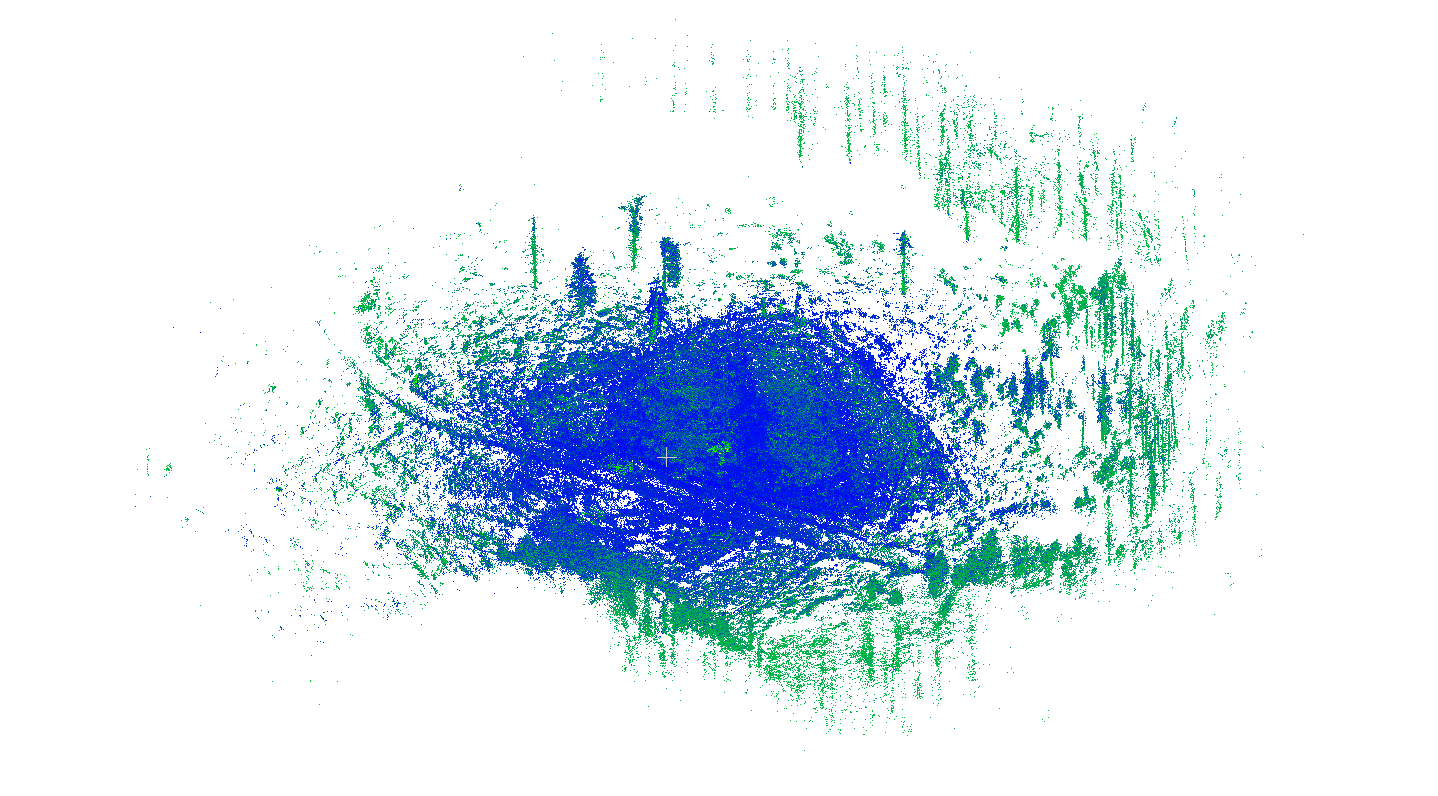
\includegraphics[width=0.4\textwidth]{rnd-project-report-main/figures/Original_data.png}
    %     \caption{Original LiDAR Data Visualization}
    % \end{figure}
    
    The figure\ref{fig:raw_data} represents a visualization of the original LiDAR point cloud data captured from a UAV-mounted sensor system over a forested area. The data is visualized using a color-coded scheme to represent different spatial distributions, where shades of blue and green indicate variations in surface elevation and structure density.
    
    The dense central region of the point cloud signifies the forest floor and lower vegetation layers, while the vertically extended, less dense structures—predominantly colored green—correspond to taller vegetation such as trees. The presence of vertical lines and scattered points further suggests canopy-level vegetation and possibly sparse outliers from surrounding terrain features or minor alignment inaccuracies.
    
    For the scope of this project, the upper vegetative regions, including the tall tree canopies and vertical outliers, were filtered out to reduce complexity and focus analysis on the forest floor and stump structures. This preprocessing step improved segmentation precision and ensured computational efficiency in the downstream tasks. The raw dataset, after filtering, served as the foundational input for subsequent preprocessing, alignment, labeling, and segmentation operations conducted throughout the study.
\begin{figure}[H]
    \centering
    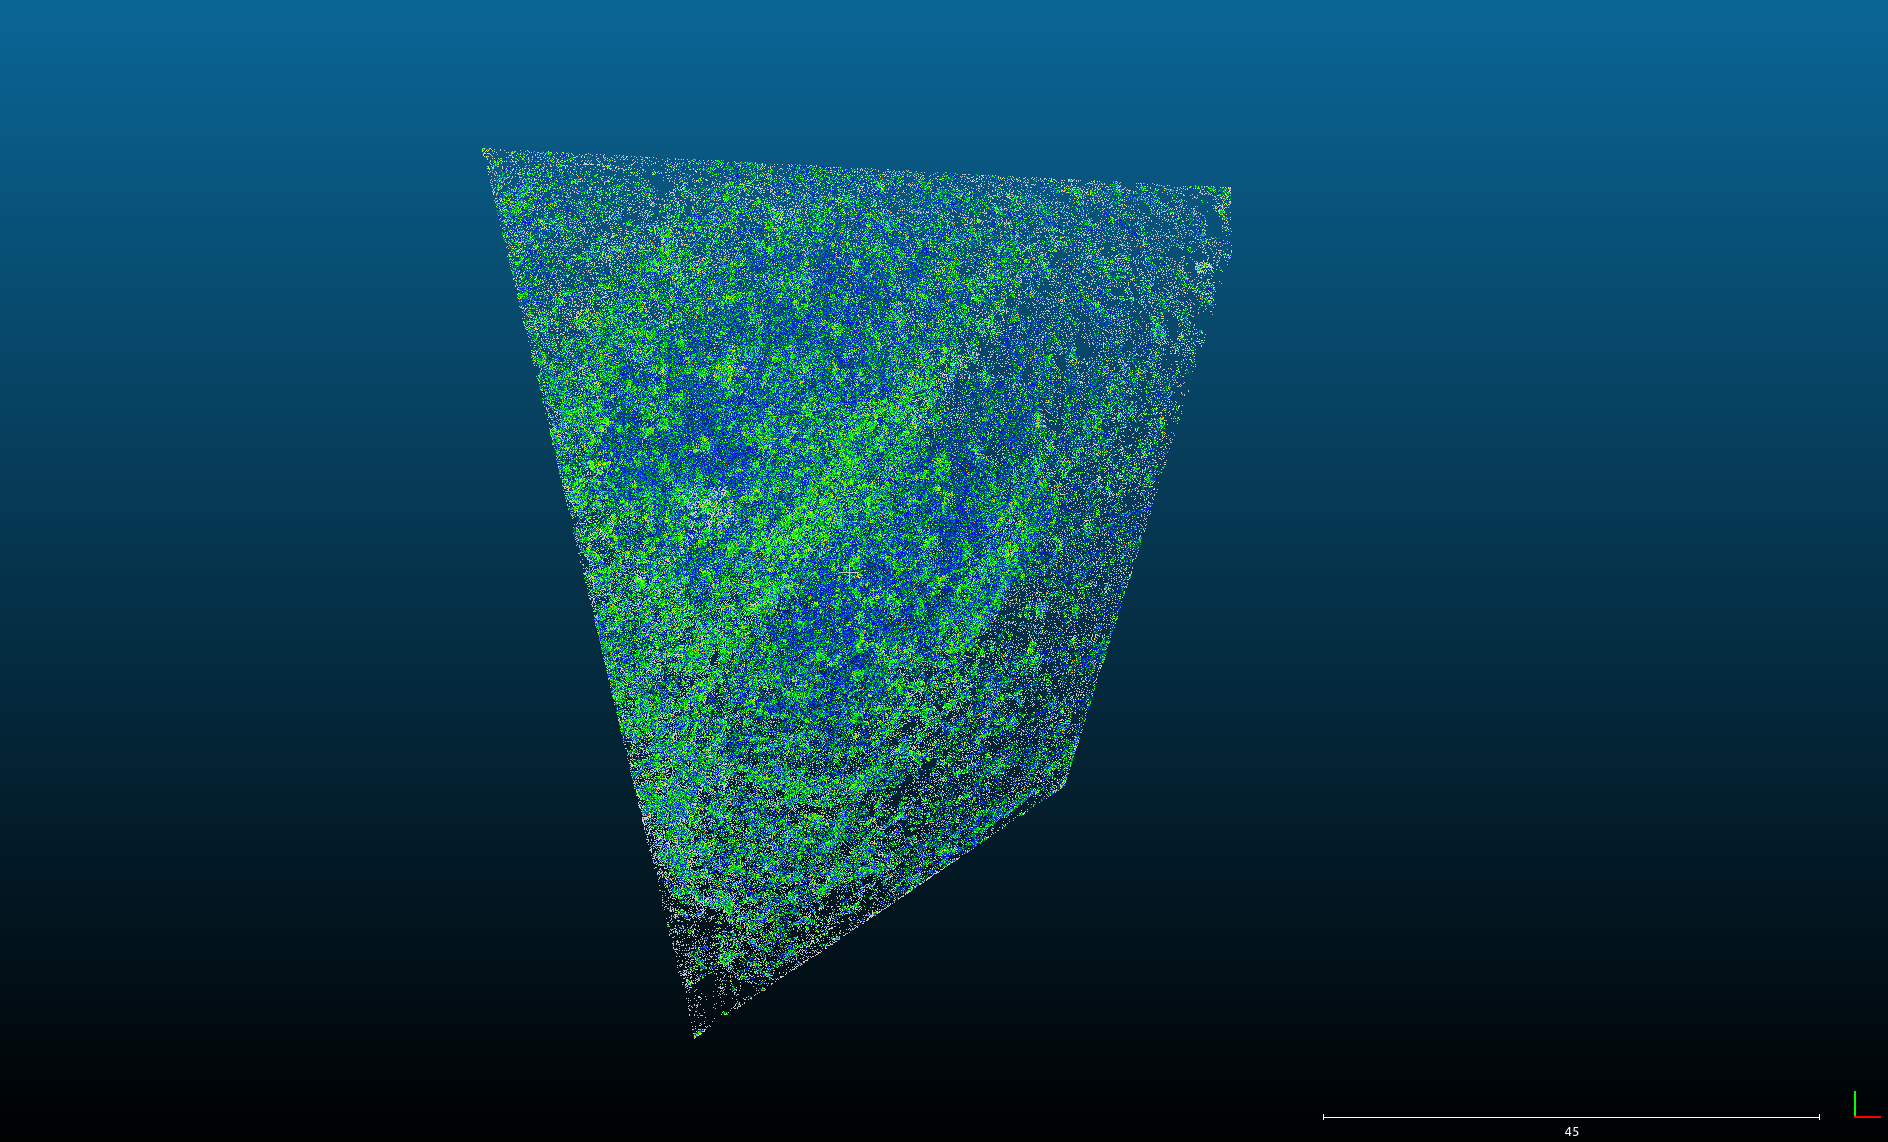
\includegraphics[width=0.4\textwidth]{rnd-project-report-main/figures/filtered_point_cloud.png}
    \caption{Filtered Point Cloud after Cropping}
\end{figure}

    \subsection{DBScan Trials}
    \begin{figure}[H]
        \centering
        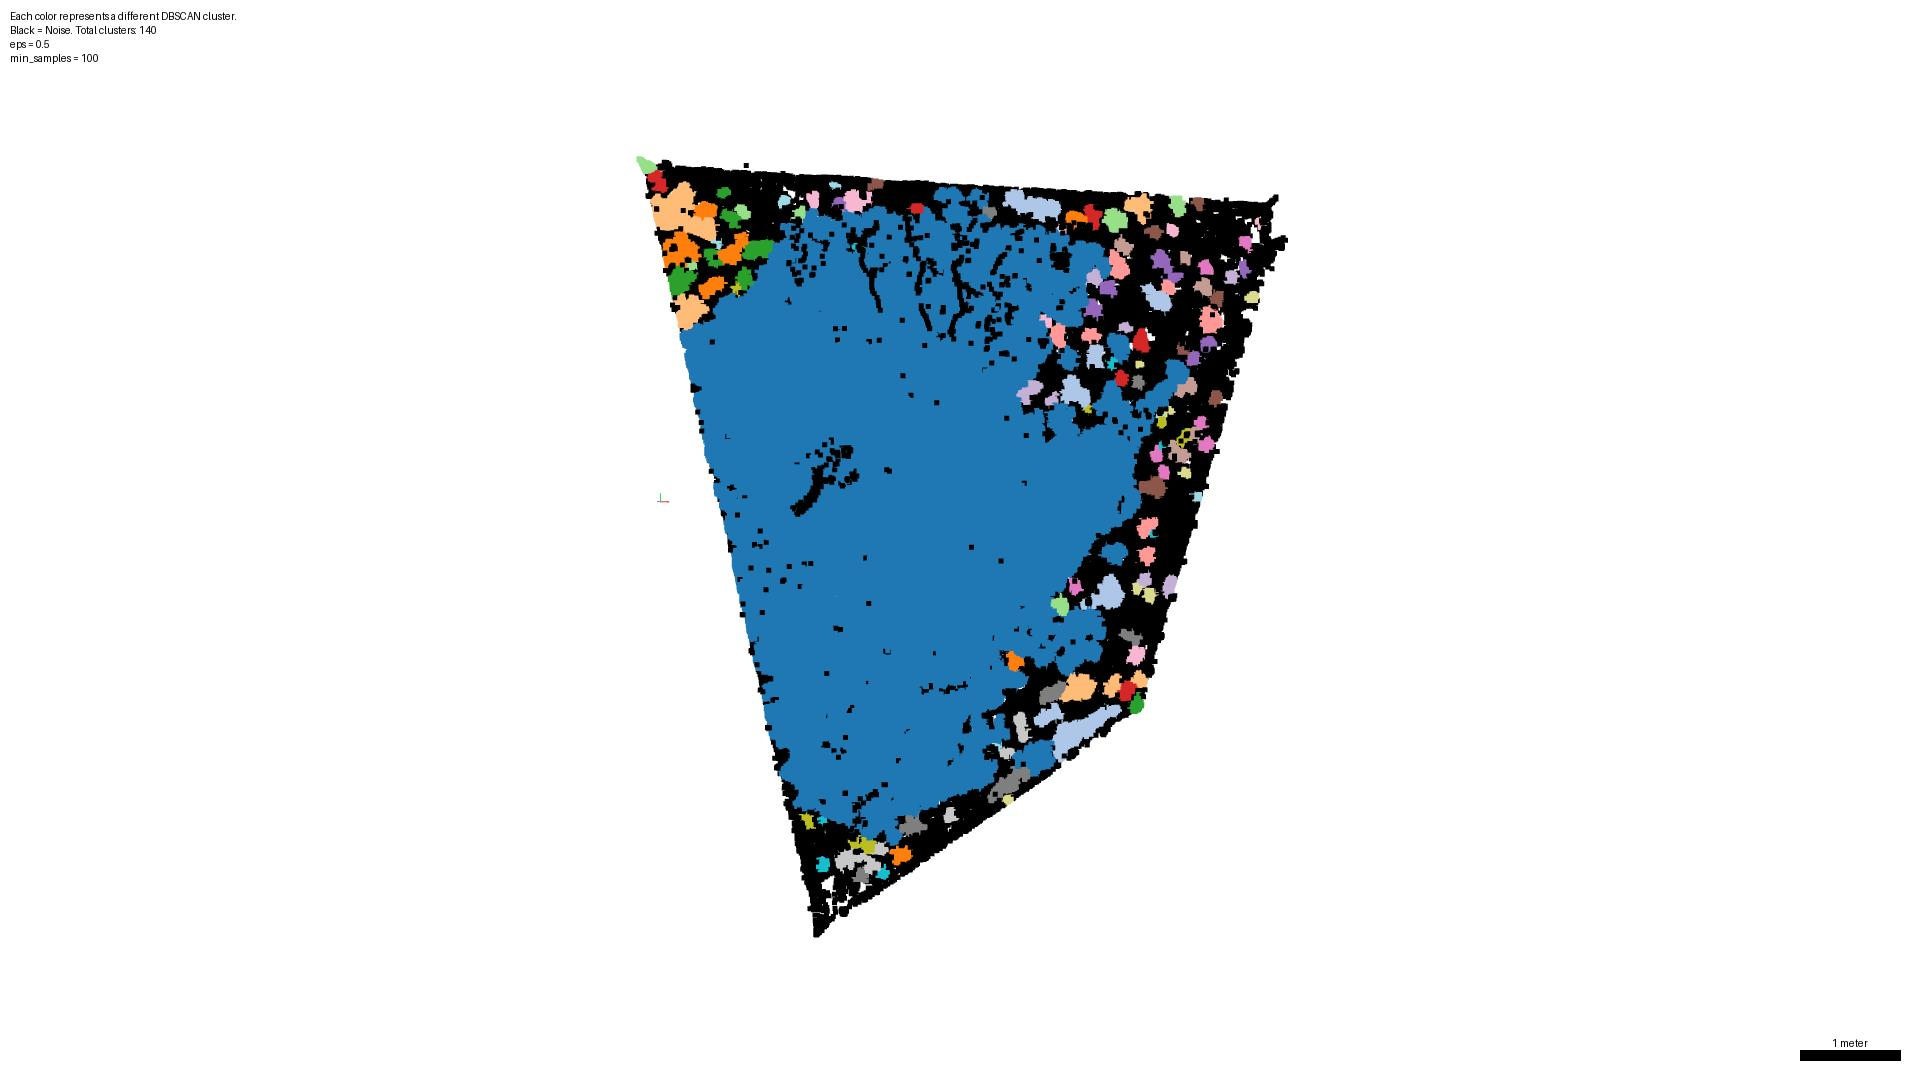
\includegraphics[width=0.4\textwidth]{rnd-project-report-main/figures/clustered_output_with_scale.jpg}
        \caption{DBScan Trial}
    \end{figure}
    DBSCAN clustering was applied to the filtered point cloud to identify spatially coherent regions that may correspond to individual stumps or other ground-level structures. The algorithm was configured with an epsilon value of 0.5 and a minimum sample threshold of 100, chosen empirically to balance between noise reduction and meaningful cluster formation. These parameters allowed for the effective segmentation of densely packed structures while filtering out sparse and isolated points as noise. The resulting cluster labels were visualized using a colormap, facilitating an intuitive assessment of spatial distribution and clustering quality. To aid spatial orientation, a reference coordinate axis was included in the visualization, enhancing interpretability within the three-dimensional scene.

    The clustering process resulted in 631 distinct clusters, not accounting for noise. These clusters captured the fine-grained structural diversity of the forest floor, highlighting the natural complexity present in such environments. The segmentation provided by DBSCAN enabled the targeted extraction of relevant subregions, such as the largest or most densely populated clusters. This output was essential for downstream analytical tasks, including object-specific feature extraction, supervised classification, and point-wise segmentation. By isolating coherent spatial groups, the DBSCAN results significantly contributed to the robustness and interpretability of subsequent modeling stages.

    \begin{figure}[H]
        \centering
        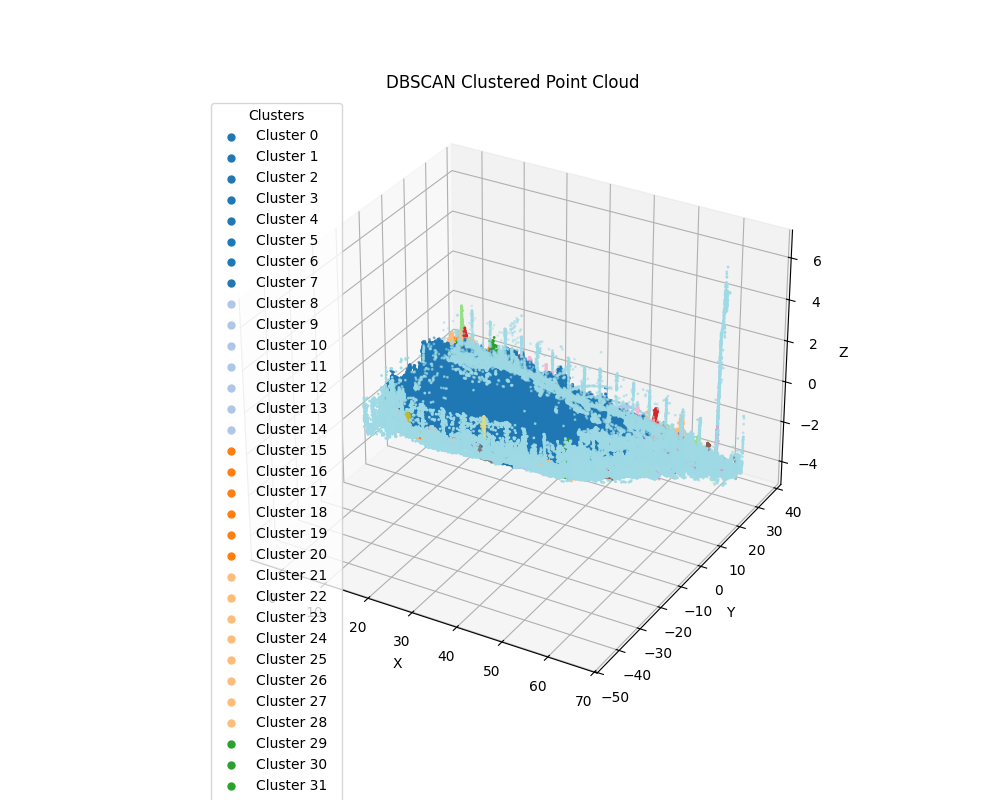
\includegraphics[width=0.4\textwidth]{rnd-project-report-main/figures/Clustering_2_filtered_point_cloud_with labels.png}
        \caption{DBScan Cylinder-like Clusters}
    \end{figure}
    Following the initial DBSCAN clustering, a geometric model-based filtering approach was employed to further refine the segmentation results. A reference cylindrical model with a radius of 150 mm and a height of 150 mm—corresponding to typical stump dimensions—was defined as a geometric constraint. Each identified cluster from the DBSCAN output was evaluated against this reference model to determine similarity based on shape and scale. Only those clusters that exhibited geometric compatibility with the reference cylinder were retained for further analysis.

    This selective filtering process yielded a total of 140 clusters that conformed to the specified cylindrical profile. These clusters are considered potential stump candidates, exhibiting structural characteristics consistent with the expected dimensions. The application of this model-based filtering step significantly reduced false positives and contributed to a more precise identification of relevant ground-level structures, thereby enhancing the accuracy of subsequent classification and segmentation tasks.

    \subsection{RANSAC}
    \begin{figure}[H]
        \centering
        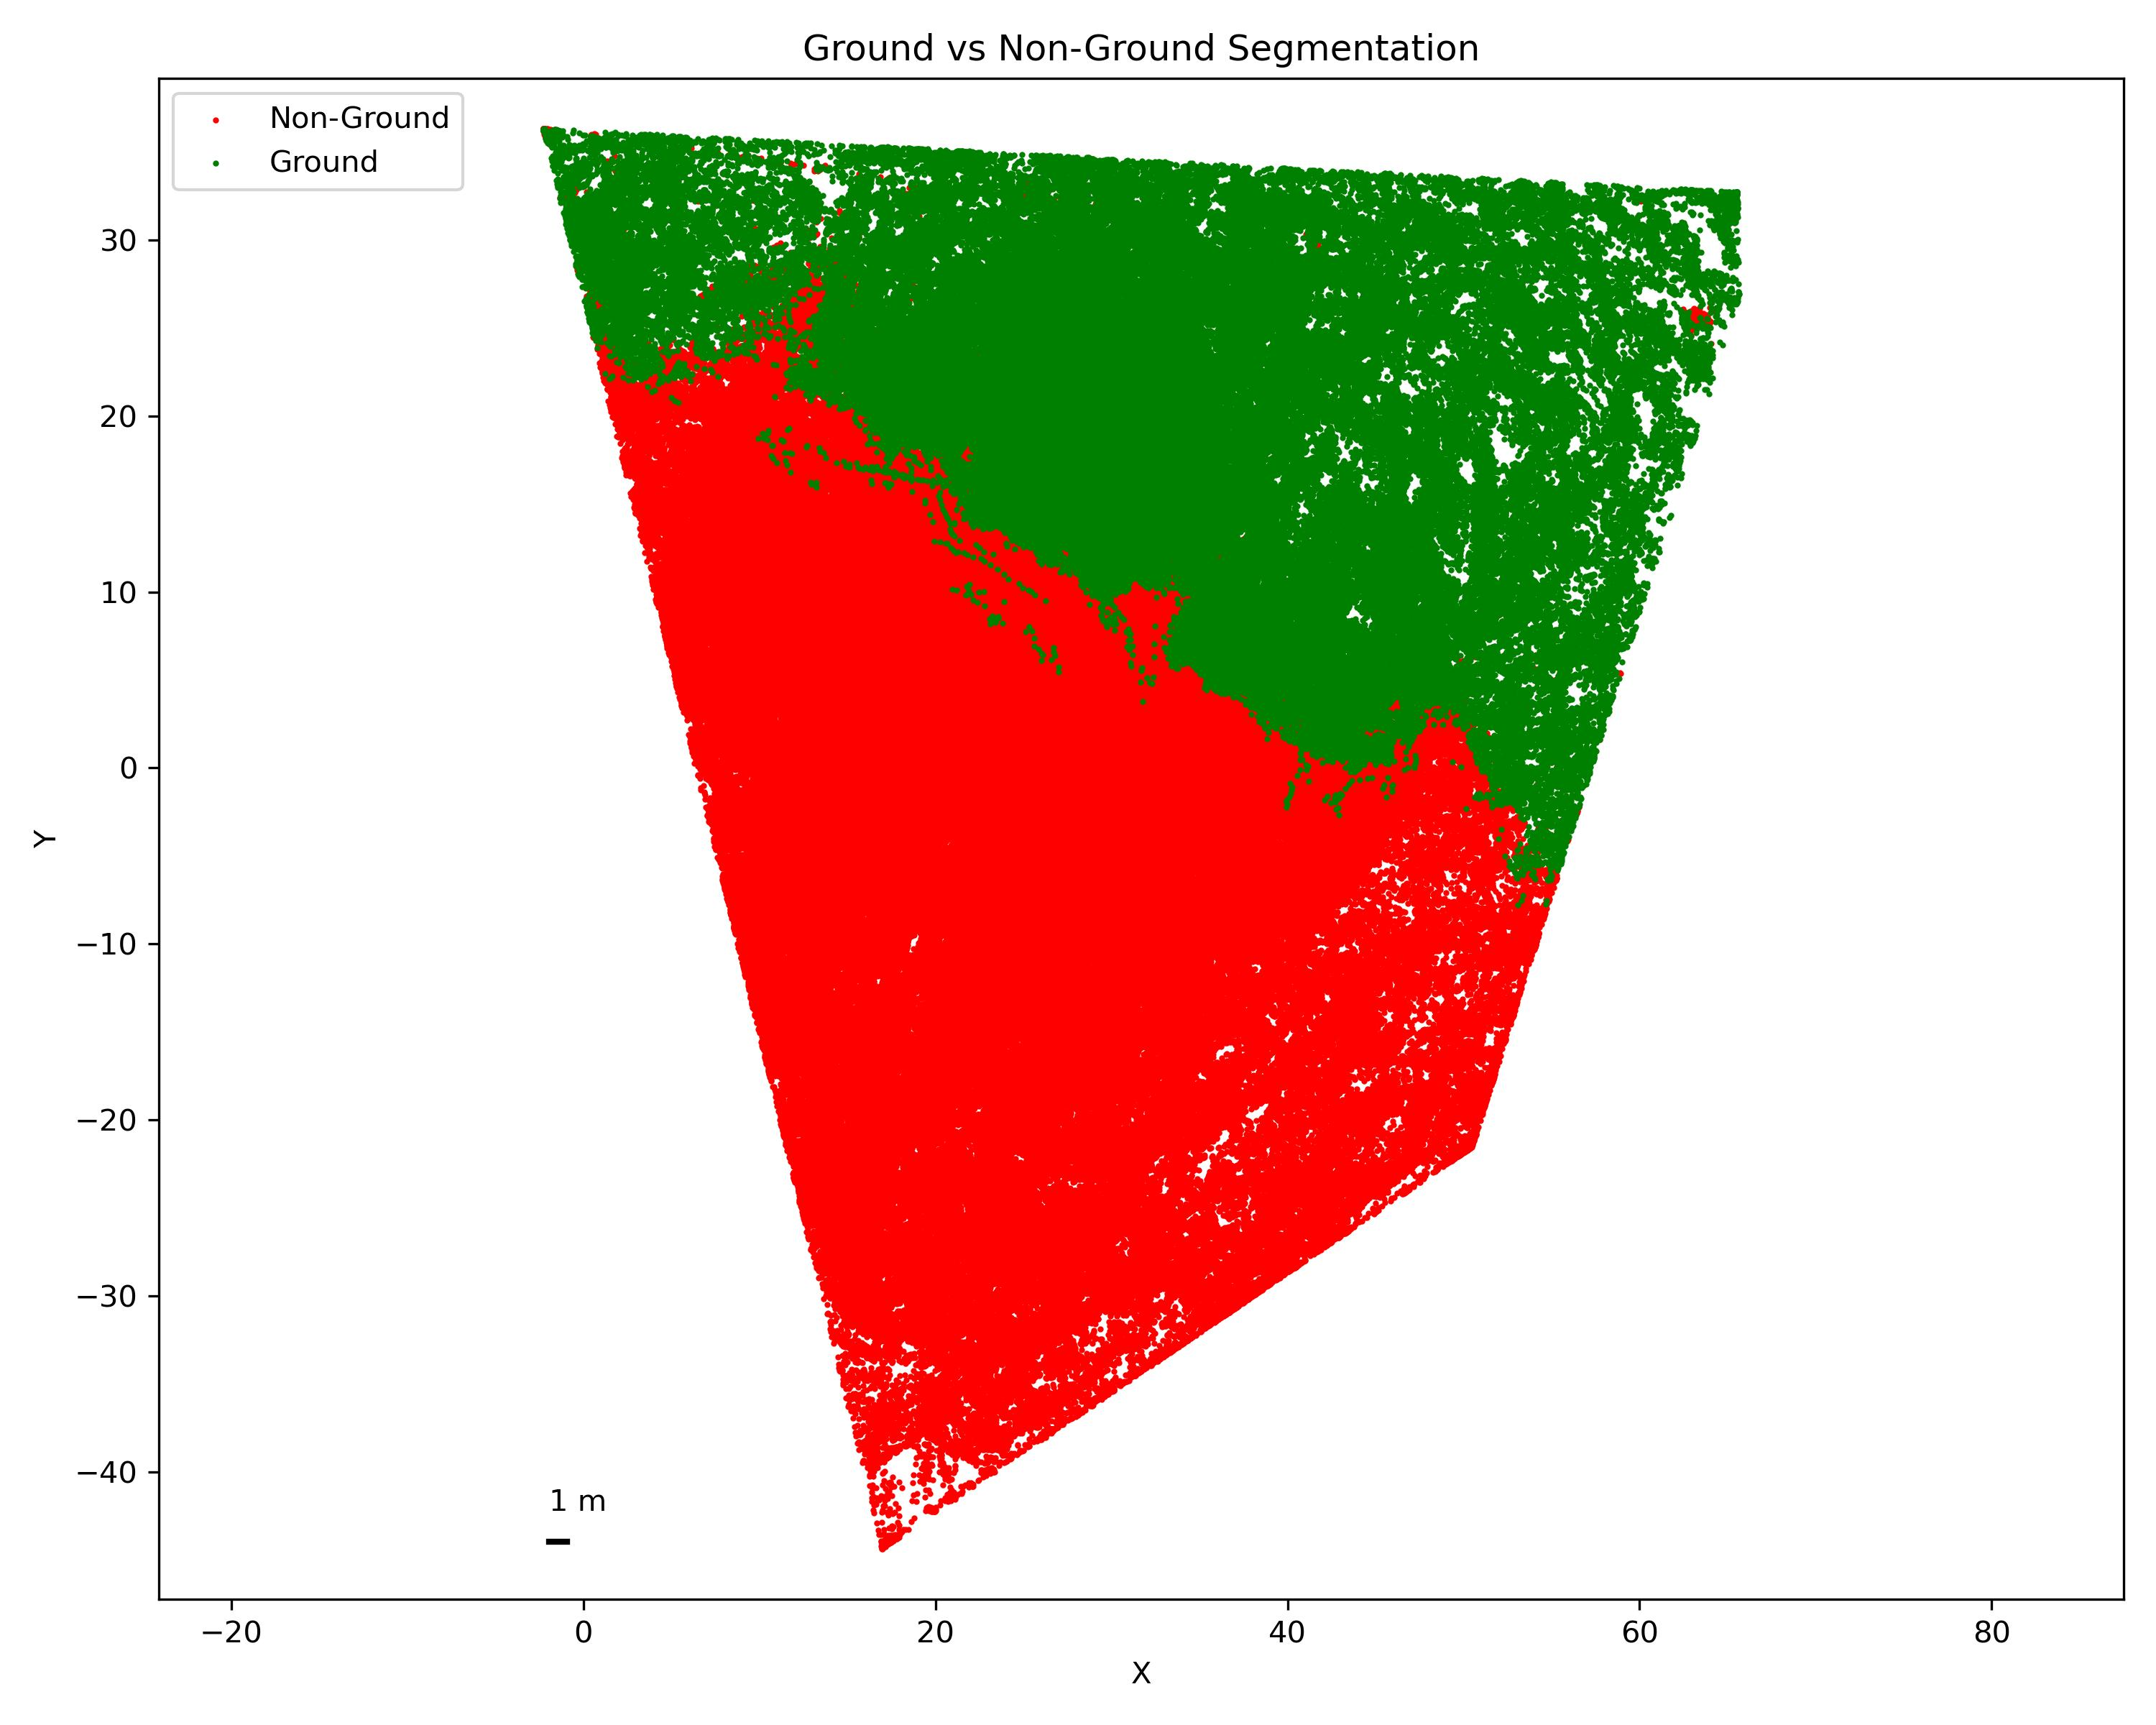
\includegraphics[width=0.4\textwidth]{rnd-project-report-main/figures/ground_non_ground_with_legend.jpg}
        \caption{RANSAC Result - Top View}
    \end{figure}
    
    The segmentation of ground and non-ground points within the forest point cloud was conducted using two complementary methodologies: a supervised learning strategy employing a Random Forest Classifier and a model-based approach utilizing RANSAC plane fitting.
    
    In the supervised classification method, a Random Forest algorithm was employed to distinguish between terrain and non-terrain features based on geometric attributes including spatial coordinates and curvature. Ground-truth labels were derived using the 25th percentile of the Z-axis distribution, providing a robust criterion for terrain estimation. Prior to training, the dataset underwent normalization to ensure consistent feature scaling. The classifier processed a total of 145,134 points, successfully identifying 36,413 as ground and 108,721 as non-ground. The segmentation results were visualized, with ground points represented in green and non-ground points in red, effectively delineating terrain surfaces from above-ground vegetation and structures.
    
    Simultaneously, a model-based technique employing RANSAC (Random Sample Consensus) was implemented to estimate the underlying ground surface. This algorithm iteratively fits a plane to the point cloud data by selecting subsets of points and evaluating inlier consensus within a defined distance threshold. Points lying within this threshold from the estimated plane were classified as ground (green), while remaining points were categorized as non-ground (red).
    
    Both segmentation strategies yielded high-quality results that are visually interpretable and suitable for further analysis. The Random Forest-based approach provided reliable and quantitatively robust visual performance. In contrast, the RANSAC approach served as a geometric validation technique, offering a model-driven alternative that effectively captured the planar characteristics of the forest floor. Together, these methods present a comprehensive framework for terrain extraction from LiDAR-based point cloud data in forested environments.
    
\subsection{PointNet Classification}
\begin{figure}[H]
    \centering
    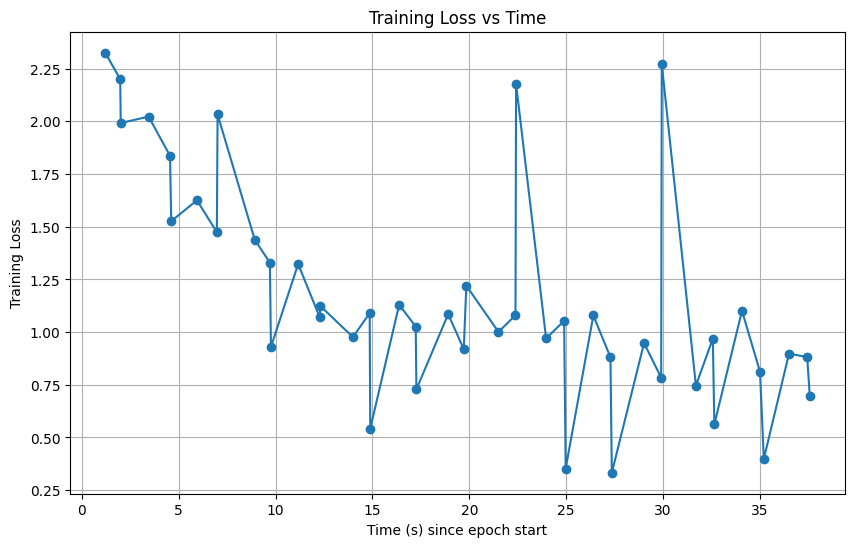
\includegraphics[width=0.4\textwidth]{rnd-project-report-main/figures/PointNetClass.png}
    \caption{PointNetClass output}
\end{figure}
        \noindent\textbf{Test accuracy:  59.73\%}
    
    In the classification task, the dataset utilized was in the .off file format, which encapsulates mesh information comprising vertices and faces for each sample representing classes such as terrain, stumps, and miscellaneous objects. While the inclusion of face data alongside vertices provides a richer geometric context, integrating face features directly into the PointNet architecture introduced challenges. PointNet is inherently designed to process unordered point sets, and the structured nature of mesh faces conflicted with this requirement, leading to inconsistencies during training and a potential reduction in classification precision.\cite{pointnetclass}
    
    To address this, synthetic faces were generated based on the vertices alone, enabling a more uniform and consistent feature set across the dataset. This approach allowed the classifier to leverage structural information derived from the spatial configuration of points without introducing irregularities associated with original mesh face data. As a result, the training process was stabilized and model performance improved in terms of classification accuracy and generalization. This refinement enhanced the effectiveness of PointNet in distinguishing between different structural categories present in the forest environment.
    
\subsection{PointNet++ Segmentation}

\begin{figure}
    \centering
    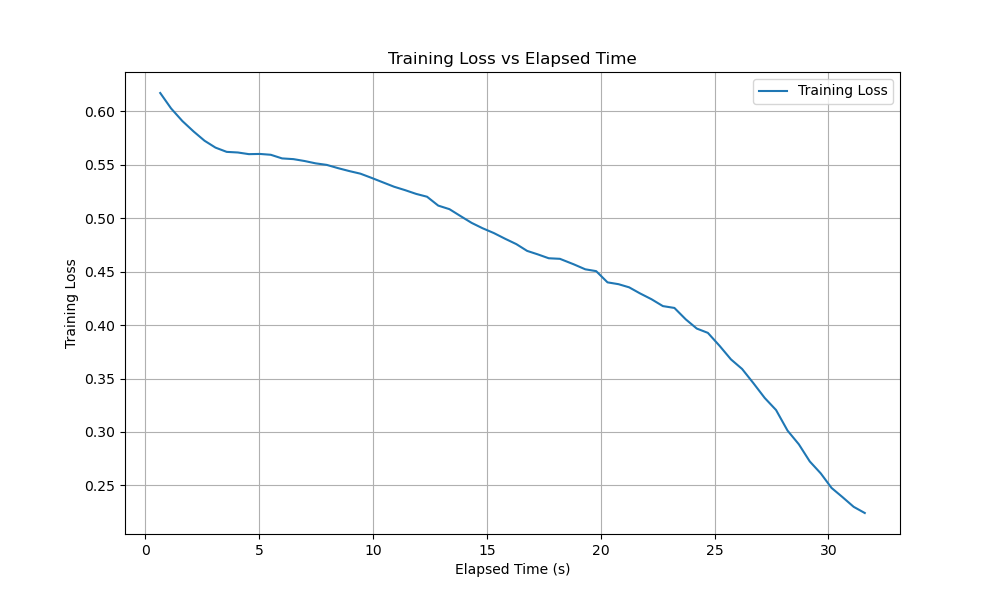
\includegraphics[width=0.4\textwidth]{rnd-project-report-main/figures/PointNetSeg_output.png}
    \caption{PointNet++ Segmentation Batch Size - 128, Epochs - 64}
\end{figure}


\begin{figure}
    \centering
    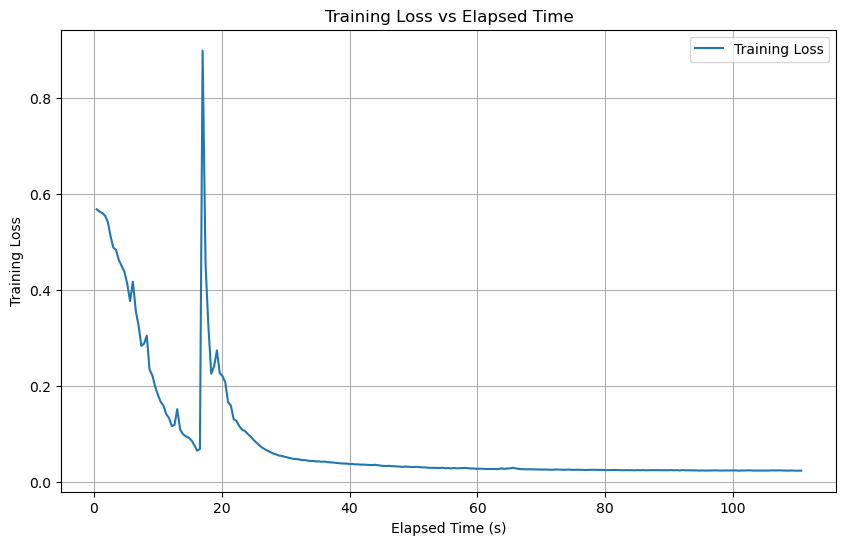
\includegraphics[width=0.7\linewidth]{rnd-project-report-main/figures/PointNetSeg_bs128_ep251.png}
    \caption{PointNet++ Segmentation Batch Size - 128, Epochs - 251}
    \label{fig:pointnetseg_bs128_ep251}
\end{figure}

\begin{figure}
    \centering
    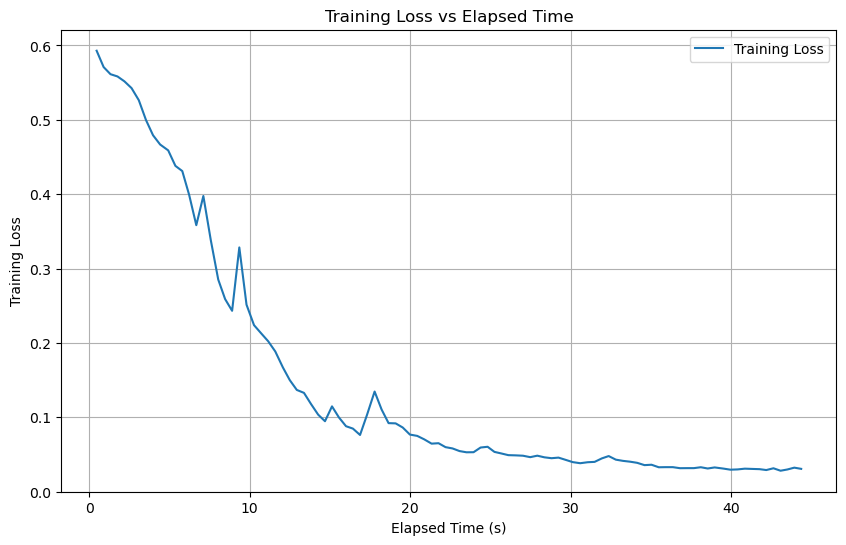
\includegraphics[width=0.7\linewidth]{rnd-project-report-main/figures/PointNetSeg_bs128.png}
    \caption{PointNet++ Segmentation Batch Size - 128}
    \label{fig:pointnetseg_bs128}
\end{figure}


\begin{table}[h!]
\centering
\caption{Test Accuracy of PointNet++ Segmentation Models}
\begin{tabular}{|l|c|c|c|c|}
\hline
\textbf{Trial} & \textbf{Batch Size} & \textbf{Epochs} & \textbf{Test Accuracy} & \textbf{Reference Graph} \\
\hline
CSF & 128 & 251 & 34.14\% & Figure~\ref{fig:pointnetseg_bs128_ep251} \\
CSF & 128 & 100   & 36.15\% & Figure~\ref{fig:pointnetseg_bs128} \\
Grids & 128   & 64   & 86.77\% & Figure~\ref{fig:pointnetseg_grids} \\

\hline
\end{tabular}
\label{tab:pointnet_results}
\end{table}

In the segmentation phase, the dataset was spatially divided into grid-based subregions to facilitate localized processing and annotation. Each grid segment was labeled into one of three predefined classes: terrain, stump, and non-terrain or everything else. Two distinct terrain extraction approaches were employed to generate ground truth for segmentation.

The first method utilized RANSAC-based plane fitting to identify terrain points. This approach estimated the ground surface by fitting a planar model and labeling points within a certain proximity to this surface as terrain. All remaining points above the threshold were considered non-terrain. The second approach employed the Cloth Simulation Filter (CSF), a model inspired by cloth physics, to simulate a draped surface over the point cloud. Points below this simulated cloth were classified as terrain, while the rest were treated as non-terrain.

Following terrain extraction, the segmented point clouds were further refined by identifying stump-like structures from previously extracted .ply files. These were algorithmically labeled and assigned a class index of 1, while terrain points were labeled as 0. All remaining non-terrain points—either identified through RANSAC or CSF—were grouped under the class label 2. This structured labeling enabled effective training and evaluation of segmentation models across diverse forest structures.\cite{Pytorch_Pointnet_Pointnet2}

\begin{table}[h!]
\centering

\begin{tabular}{cccccc}
\toprule
X & Y & Z & Label & Curvature & Density \\
\midrule
16.36002731 & 17.04719353 & -1.00251257 & 1.0 & 0.0 & 0.0 \\
\bottomrule
\end{tabular}
\caption{Sample point cloud data with features}
\label{tab:datasample}
\end{table}

\begin{figure}
    \centering
    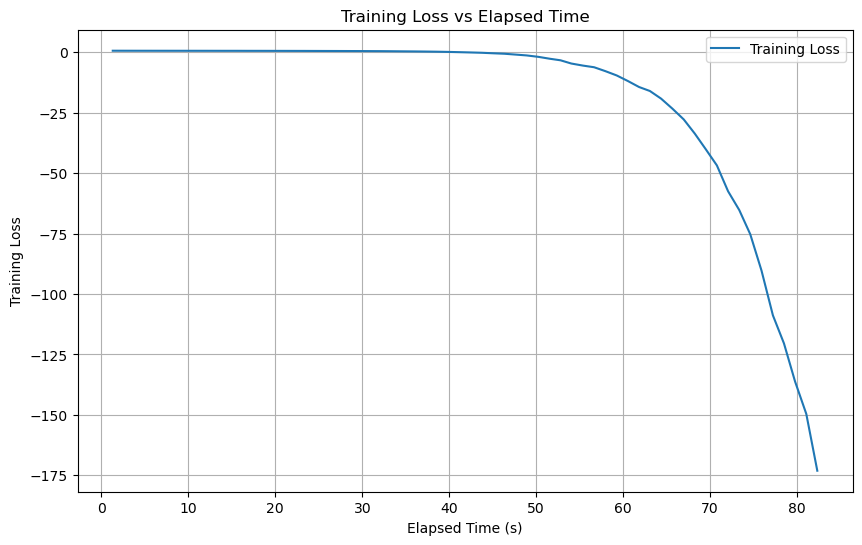
\includegraphics[width=0.7\linewidth]{rnd-project-report-main/figures/PointNetSeg_grids.png}
    \caption{PointNetSeg grids}
    \label{fig:pointnetseg_grids}
\end{figure}
    %\noindent\textbf{Test Accuracy: 86.77%}
\end{document}